\textbf{What is data science?}
With the major technological advances of the last two decades, coupled in part with the internet explosion, a new breed of analysist has emerged. The exact role, background, and skill-set, of a 
\emph{data scientist} are still in the process of being defined and it is likely that by the time you read this some of what we say will seem archaic. 

In very general terms, we view a data scientist as an individual who uses current computational techniques to analyze data.  Now you might make the observation that there is nothing particularly novel 
in this, and subsequenty ask what has forced the definition.\footnote{William S. Cleveland decide to coin the term \emph{data science} and write  \emph{Data Science: An action plan for expanding the technical areas of the field of statistics} \cite{ClevelandData}.  His report outlined six points for a university to follow in developing a data analyst curriculum.}  After all statisticians, physicists, biologisitcs, finance quants, etc have been looking at data since their respective fields 
emerged. 
One short answer comes from the fact that the data sphere has changed and, hence, a new set of skills is 
required to navigate it effectively. The exponential increase in computational power has provided new means to investigate the ever growing amount of data being collected every second of the
day. What this implies is the fact that any modern data analyst will have to make the time investment to learn computational techniques necessary to deal with the volumes and complexity of the data of today.
In addition to those of mathemics and statistics, these software skills are domain transfereable and so it makes sense to create a job title that is also transferable.  We could also point to the ``data hype'' created in industry as a culprit for the term \emph{data science} with the \emph{science} creating an aura of validity and facilitating LinkedIn headhunting.

\textbf{What skills are needed?}
One neat way we like to visualize the data science skill set is with Drew Conway's Venn Diagram\cite{ConwayVenn}, see figure \ref{figure:conwayvenn}.
\begin{figure}
  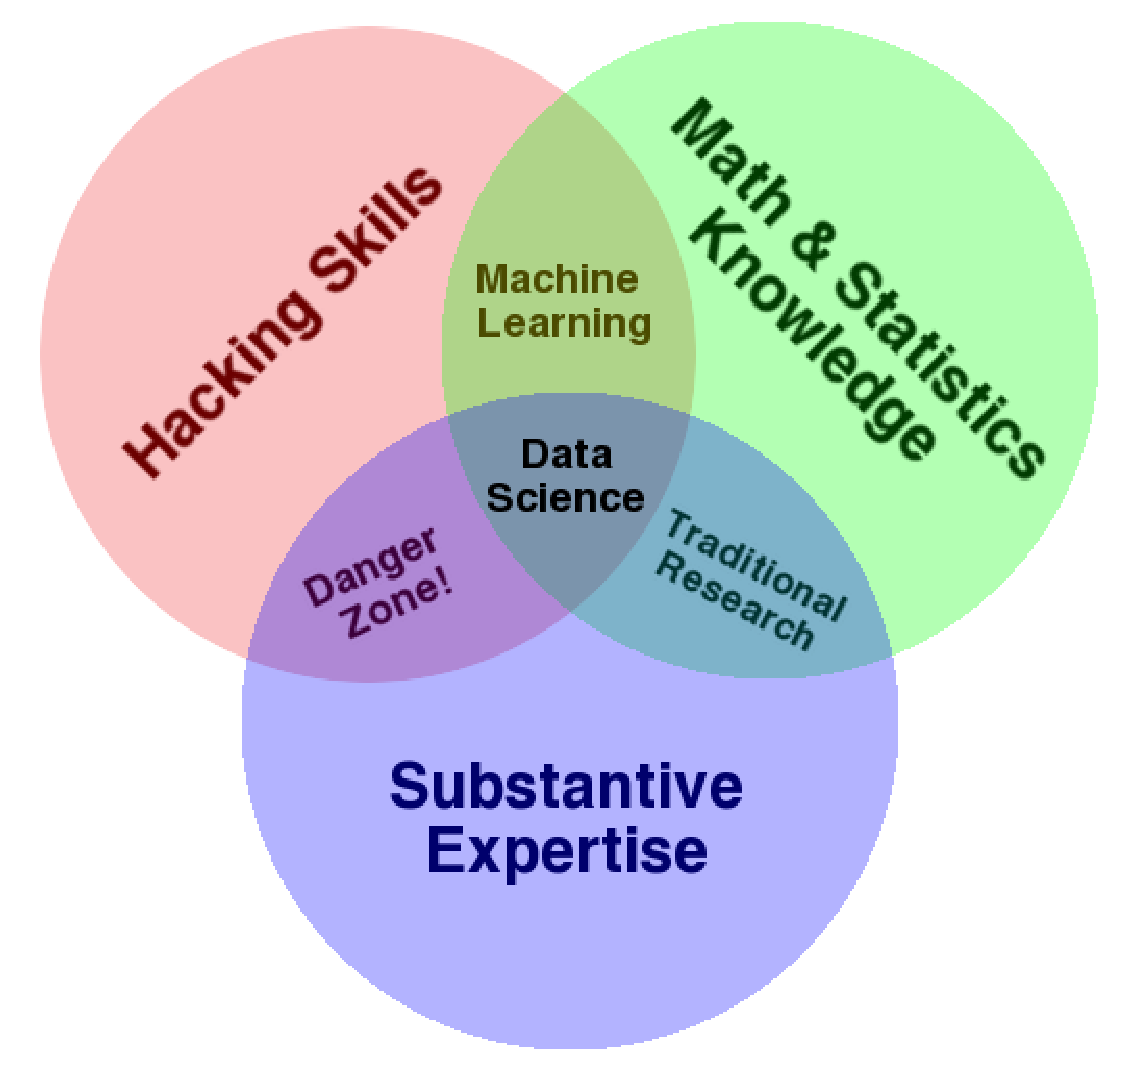
\includegraphics[width=0.5\textwidth]{../images/Data_Science_VD}
  \caption{Drew Conway's Venn Diagram}
  \label{figure:conwayvenn}
\end{figure}
Math and statistics is what allows us to properly quantify a phenomenon observed in data. For the sake of narrative lets take a complex deterministic situation, such as whether or not someone will make a loan payment, 
and attempt to answer this question with a limited number of variables and an imperfect understanding of those variables influence on the event we wish to predict. 
With the exception of your friendly real estate agent we generally acknowldege our lack of soothseer ability and make statements about the probability of this event.  These statements take a mathematical form, for example
\begin{align*}
  \rmP[\mbox{makes-loan-payment}] &= e^{\alpha + \beta\cdot\mbox{creditscore}}.
\end{align*}
where the above quantifies the \emph{risk} associated with this event.  Deciding on the best coefficients $\alpha$ and $\beta$ can be done quite easily by a host of software packages.  In fact anyone with decent hacking
skills can do achieve the goal.  Of course, a simple model such as this would convince no one and would call for substantive expertise (more commonly called \emph{domain knowledge}) to make real progress.  In this case, 
a domain expert would note that additional variables such as the loan to value ratio and housing price index are needed as they have a huge effect on payment activity. These variables and many others 
would allow us to arrive at a  ``better'' model
\begin{align}
  \rmP[\mbox{makes-loan-payment}] &= e^{\alpha + \beta\cdot X}.
  \label{align:preface:logit}
\end{align}
Finally we have arrived at a model capable of fooling someone!  We could keep adding  variables until the model will almost certainly fit the historic risk quite well.  BUT, how do we know that this will allow us to quantify risk in the future? 
To make some sense of our \emph{uncertainty}\footnote{The distrinction between uncertainty and risk has been talked about quite extensively by Nassim Taleb\cite{TalebFooled,TalebBlack}} about our model we need to know eactly what
\eqref{align:preface:logit} means.   In particular, did we include too many variables and \emph{overfit}?  Did our method of solving \eqref{align:preface:logit} arrive at a good solution or just numerical noise?  Most importantly, 
how appropriate is the logistic regression model to begin with?  Answering these questions is often as much an art as a science, but in our experience, sufficient mathematical understanding is necessary to avoid getting lost.


\textbf{What is the motivation for, and focus of, this course?}
Just as common as the hacker with no domain knowledge, or the domain expert with no statistical no-how is the traditional academic with meager computing skills.  Academia rewards papers containing original theory.  For the most part 
it does not reward the considerable effort needed to produce high quality, maintainable code that can be used by others and integrated into larger frameworks.  
As a result, the type of code typically put forward by academics is completely unuseable in industry or by anyone else for that matter. It is often not the purpose or worth the effort to write production level code
in an academic environment. The importance of this cannot be overstated.  Consider a 20 person start-up that wishes to build a smart-phone app that recommends restaurants to users.  
The data scientist hired for this job will need to interact with the company database (they will likely not be handed a neat csv file), deal with falsely entered or inconveniently formatted data, and produce legible reports, 
as well as a working model for the rest of the company to integrate into its production framework. The scientist may be expected to do this work without much in the way of software support.  Now, considering how easy it is to 
blindly run most predictive software, our hypothetical company will be tempted to use a programmer with no statistical knowledge to do this task.  Of course, the programmer will fall into analytic traps such as the ones mentioned above but 
that might not deter anyone from being content with output. This anecdote seems construed, but in reality it is something we have seen time and time again. The current world of data analysis calls for a myriad of skills, 
and clean programming, database interaction and understand of architecture have all become the minimum to succeed. 

The purpose of this course is to take people with strong mathematical/statistical knowledge and teach them software development fundamentals\footnote{Our view of what constitutes the necessary fundamentals is strongly influenced by the team at software carpentry\cite{SWC}}.  This course will cover
\begin{itemize}
  \item Design of small software packages
  \item Working in a Unix environment
  \item Designing software in teams
  \item Fundamental statistical algorithms such as linear and logistic regression
  \item Overfitting and how to avoid it
  \item Working with text data (e.g. regular expressions)
  \item Time series
  \item And more\dots
\end{itemize}

